\documentclass[journal,12pt,twocolumn]{IEEEtran}
%

\usepackage{setspace}
\usepackage{gensymb}
\singlespacing

\usepackage{amsmath}
\usepackage{amsthm}
\usepackage{txfonts}
\usepackage{cite}
\usepackage{enumitem}
\usepackage{mathtools}
\usepackage{listings}
    \usepackage{color}                                            %%
    \usepackage{array}                                            %%
    \usepackage{longtable}                                        %%
    \usepackage{calc}                                             %%
    \usepackage{multirow}                                         %%
    \usepackage{hhline}                                           %%
    \usepackage{ifthen}                                           %%
  %optionally (for landscape tables embedded in another document): %%
    \usepackage{lscape}     
\usepackage{multicol}
\usepackage{chngcntr}
\usepackage[center]{caption}
\renewcommand\thesection{\arabic{section}}
\renewcommand\thesubsection{\thesection.\arabic{subsection}}
\renewcommand\thesubsubsection{\thesubsection.\arabic{subsubsection}}

\renewcommand\thesectiondis{\arabic{section}}
\renewcommand\thesubsectiondis{\thesectiondis.\arabic{subsection}}
\renewcommand\thesubsubsectiondis{\thesubsectiondis.\arabic{subsubsection}}

% correct bad hyphenation here
\hyphenation{op-tical net-works semi-conduc-tor}
\def\inputGnumericTable{}                                 %%

\lstset{
%language=C,
frame=single, 
breaklines=true,
columns=fullflexible
}

\begin{document}
%


\newtheorem{theorem}{Theorem}[section]
\newtheorem{problem}{Problem}
\newtheorem{proposition}{Proposition}[section]
\newtheorem{lemma}{Lemma}[section]
\newtheorem{corollary}[theorem]{Corollary}
\newtheorem{example}{Example}[section]
\newtheorem{definition}[problem]{Definition}
\newcommand{\BEQA}{\begin{eqnarray}}
\newcommand{\EEQA}{\end{eqnarray}}
\newcommand{\define}{\stackrel{\triangle}{=}}

\bibliographystyle{IEEEtran}


\providecommand{\mbf}{\mathbf}
\providecommand{\pr}[1]{\ensuremath{\Pr\left(#1\right)}}
\providecommand{\qfunc}[1]{\ensuremath{Q\left(#1\right)}}
\providecommand{\sbrak}[1]{\ensuremath{{}\left[#1\right]}}
\providecommand{\lsbrak}[1]{\ensuremath{{}\left[#1\right.}}
\providecommand{\rsbrak}[1]{\ensuremath{{}\left.#1\right]}}
\providecommand{\brak}[1]{\ensuremath{\left(#1\right)}}
\providecommand{\lbrak}[1]{\ensuremath{\left(#1\right.}}
\providecommand{\rbrak}[1]{\ensuremath{\left.#1\right)}}
\providecommand{\cbrak}[1]{\ensuremath{\left\{#1\right\}}}
\providecommand{\lcbrak}[1]{\ensuremath{\left\{#1\right.}}
\providecommand{\rcbrak}[1]{\ensuremath{\left.#1\right\}}}
\theoremstyle{remark}
\newtheorem{rem}{Remark}
\newcommand{\sgn}{\mathop{\mathrm{sgn}}}
\providecommand{\abs}[1]{\left\vert#1\right\vert}
\providecommand{\res}[1]{\Res\displaylimits_{#1}} 
\providecommand{\norm}[1]{\left\lVert#1\right\rVert}
\providecommand{\mtx}[1]{\mathbf{#1}}
\providecommand{\mean}[1]{E\left[ #1 \right]}
\providecommand{\fourier}{\overset{\mathcal{F}}{ \rightleftharpoons}}
\providecommand{\system}{\overset{\mathcal{H}}{ \longleftrightarrow}}
\newcommand{\solution}{\noindent \textbf{Solution: }}
\newcommand{\cosec}{\,\text{cosec}\,}
\providecommand{\dec}[2]{\ensuremath{\overset{#1}{\underset{#2}{\gtrless}}}}
\newcommand{\myvec}[1]{\ensuremath{\begin{pmatrix}#1\end{pmatrix}}}
\newcommand{\cmyvec}[1]{\ensuremath{\begin{pmatrix*}[c]#1\end{pmatrix*}}}
\newcommand{\mydet}[1]{\ensuremath{\begin{vmatrix}#1\end{vmatrix}}}
\newcommand{\proj}[2]{\textbf{proj}_{\vec{#1}}\vec{#2}}

\let\StandardTheFigure\thefigure
\let\vec\mathbf

\title{
EE5600 Assignment 1
}
\author{ Perabhattula Venkatesh\\AI20MTECH01004}	

\maketitle

\renewcommand{\thefigure}{\theenumi}
\renewcommand{\thetable}{\theenumi}

\begin{abstract}
This document contains the solution to a Area of triangle problem.
\end{abstract}
%
Download all python and latex codes from 
%
\begin{lstlisting}
https://github.com/venky-p/EE5600/Assignment_1
\end{lstlisting}
%
\section{Problem}
\begin{lstlisting}
Problem Set: Vector2, Example II, Problem 5
\end{lstlisting}
\renewcommand{\theequation}{\theenumi}
\begin{enumerate}[label=\thesection.\arabic*.,ref=\thesection.\theenumi]
\numberwithin{equation}{enumi}

\item Find the area of the triangle formed by the points (a, c+a), (a, c) and (-a, c-a)

\section{Solution}
We are going to solve this problem using vectors

\begin{align}
\vec{P} = \myvec{a\\c+a}, \vec{Q} =\myvec{a\\c},
\vec{R} =\myvec{-a\\c-a}
\label{3}
\end{align}

Rewriting P, Q and R as product of a matrix and a vector

\begin{align}
\vec{P}=\vec{Au}=\myvec{1&0\\1&1}\myvec{a\\c}
\end{align}

\begin{align}
\vec{Q}=\vec{Bu}=\myvec{1&0\\0&1}\myvec{a\\c}
\end{align}

\begin{align}
\vec{R}=\vec{Cu}=\myvec{-1&0\\-1&1}\myvec{a\\c}
\end{align}

\begin{align}
\text{Area of given Triangle }=\frac{1}{2}\norm{\Vec{P-Q}\times  \Vec{P-R}}
\label{1}
\end{align}

\begin{align}
\Vec{P-Q}\times  \Vec{P-R} = \vec{(Au-Bu)\times(Au-Cu)}
\end{align}

\begin{align}
=\vec{Au}\times\vec{Au}-\vec{Au}\times\vec{Cu}-\vec{Bu}\times\vec{Au}\\+\vec{Bu}\times\vec{Cu}
\end{align}
\begin{align}
=\vec{Au}\times\vec{Bu}+\vec{Bu}\times\vec{Cu}+\vec{Cu}\times\vec{Au}
\end{align}

\begin{align}
=\myvec{a\\c+a}\times\myvec{a\\c}+\myvec{a\\c}\times\myvec{-a\\c-a}+\myvec{-a\\c-a}\times\myvec{a\\c+a}
\end{align}

\begin{align}
=\myvec{0\\0\\-a^2}+\myvec{0\\0\\-a^2}+\myvec{0\\0\\0}
\end{align}

\begin{align}
=\myvec{0\\0\\-2a^2}
\label{5}
\end{align}

By Substituting \eqref{5} in \eqref{1}, We get

\begin{align}
\text{Area of given Triangle }=\frac{1}{2}\begin{Vmatrix}
0\\0\\-2a^2
\end{Vmatrix}
\end{align}

\begin{align}
= \frac{1}{2}\sqrt{0^2 + 0^2+ (-2a^2)^2}   
\end{align}

\begin{align}
= \frac{1}{2} 2a^2   
\end{align}

\begin{align}
=a^2
\end{align}

\begin{align}
\boxed{\therefore \text{Area of given Triangle }=a^2 units^2}
\label{4}
\end{align}

\section{Numerical Example}
Let,
\begin{align}
\vec{u}=\myvec{a\\c}=\myvec{2\\4}
\end{align}
\solution
By substituting the given values in \eqref{3}, We get

\begin{align}
\vec{P}=\myvec{2\\6},\vec{Q}=\myvec{2\\4},\vec{R}=\myvec{-2\\2}
\end{align}

\begin{figure}[h]
	\centering
	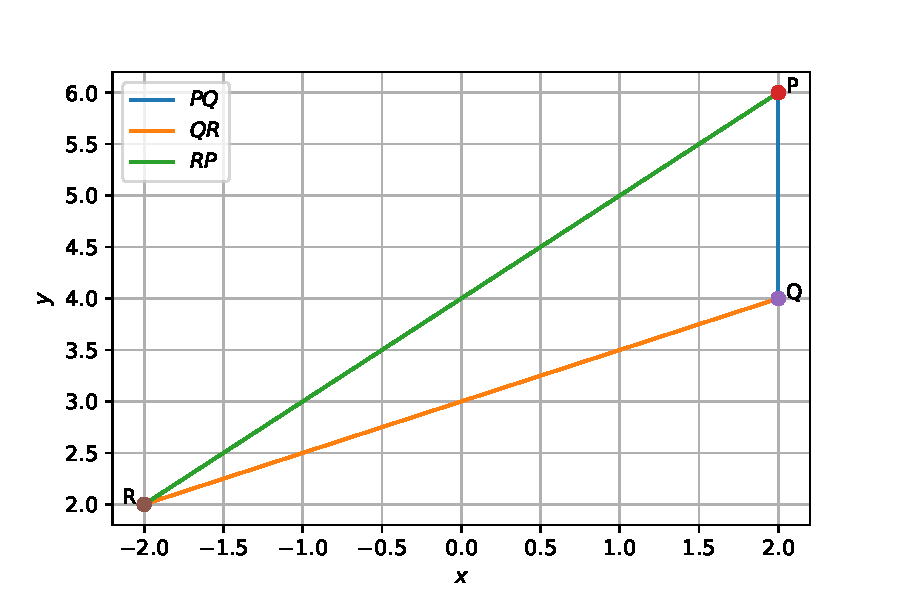
\includegraphics[width=\columnwidth]{Figure_1.pdf}
	\caption{Plot obtained from Python code}
	\label{Fig:3.1}
\end{figure}

Using \eqref{4},
\begin{align}
\text{Area of given Triangle }=a^2\\=2^2\\=4 units^2
\end{align}

\end{enumerate}

\end{document}


